\documentclass[12pt,a4paper, oneside]{article}
\usepackage[utf8]{inputenc}
\usepackage[T1]{fontenc}
\usepackage[english,german]{babel}
\usepackage[style=german]{csquotes}
\usepackage{graphicx}

\author{Uni Oldenburg, SWP2020 Gruppe A}

\begin{document}

    \begin{titlepage}
        \pagestyle{empty}
        \begin{center}

            \begin{figure}[h]
                \centering
                
\includegraphics[width=0.35\textwidth]{img/Logo.jpg}
            \end{figure}

            \bigskip \bigskip \noindent
            \textsc{\textbf{\LARGE Softwareprojekt:}} \par \bigskip \noindent
            \textsc{\textbf{\LARGE Projekttagebuch}}


            \par \bigskip \bigskip \bigskip \bigskip \bigskip \noindent
            {\Large Gruppe A} \par \medskip \noindent

            \par \bigskip \bigskip \bigskip \bigskip \bigskip \bigskip \noindent
            \textit{\Large Wintersemester 2020/21 und} \par \noindent
            \textit{\Large Sommersemester 2021}

            \par \bigskip \bigskip \bigskip \bigskip \bigskip \bigskip \noindent
            \par \bigskip \bigskip \bigskip \noindent
            {\Large Sprintanalyse} \par \medskip \noindent

        \end{center}
    \end{titlepage}

    \tableofcontents
    \pagebreak



    \section{Sprinttagebuch: Sprint-Nr. 1}
    \underline{Name des Sprints:}
    \\
    Sprint 1

    \noindent
    \\
    \underline{Zeitraum des Sprints:}
    \\
    19. November 2020 - 08. Dezember 2020

    \noindent
    \\
    \underline{Ziel des Sprints:}
    \\
    Funktionale Lobbys und Chat im Sinne ihrer User-Stories und der DoD

    \noindent
    \\
    \underline {Team:}
    \\
    Sven Ahrens, Alwin Bossert, Aldin Dervisi, Marvin Drees, Mario Fokken,
    Timo Gerken, Finn Haase, Temmo Junkhoff, Maximilian Lindner, Steven Luong, Phillip-André Suhr, Eric Vuong


    \section{Vorgänge}

    \begin{itemize}
        \item SWP2020A-33: Als Nutzer möchte ich vom Hauptmenü aus eine neue Lobby erstellen können. (8 Story Points)

        \item SWP2020A-34: Phillips Lösungen (Blatt 2, A2 und A3) einpflegen (1 Story Point)

        \item SWP2020A-46: Einfügen fehlender SuppressWarnings (UnstableApiUsage) (1 Story Point)

        \item SWP2020A-47: Als Nutzer möchte ich vom Hauptmenü einer der dort sichtbaren Lobbys beitreten können. (8 Story Points)

        \item SWP2020A-48: Als Nutzer möchte ich die existierenden Lobbys im Hauptmenü sehen können. (8 Story Points)

        \item SWP2020A-49: Als Nutzer möchte ich mit einem Button im Hauptmenü mein Passwort ändern können. (8 Story Points)

        \item SWP2020A-50: ANmi vom Fenster einer Lobby aus diese verlassen können. (5 Story Points)

        \item SWP2020A-52: Als Nutzer möchte ich eine Chatansicht sehen können. (8 Story Points)

        \item SWP2020A-53: ANmi immer die neuesten Nachrichten im Chat sehen können, damit ich der aktuellen Unterhaltung folgen kann (13 Story Points)

    \end{itemize}

    \subsection{Sprinterfolg}

    \begin{figure}[h]
        \centering
        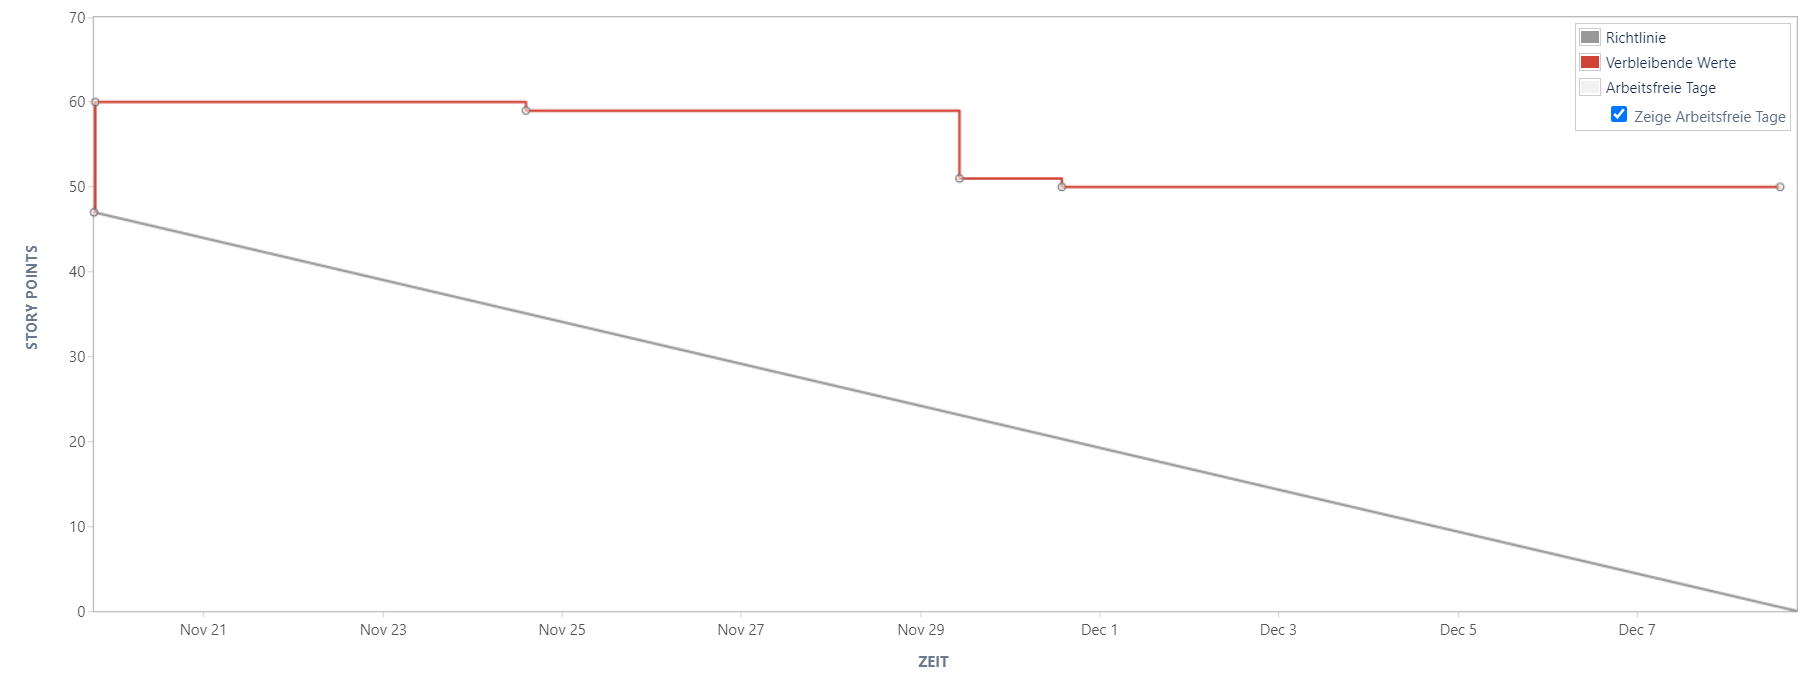
\includegraphics[width=\textwidth, height=5cm]{img/sprint_01/Burndown-Sprint1.PNG}
        \caption{Burndown-Diagramm Sprint 1}
        \label{fig: Burndown-Sprint1}
    \end{figure}

    \noindent
    Am Sprintbeginn betrug der Gesamtaufwand des Sprints 47 Story Points. Kurz nach Sprintbeginn haben wir uns entschieden, die Task \textit{SWP2020A-53: ANmi immer die neuesten Nachrichten im Chat sehen können, damit ich der aktuellen Unterhaltung folgen kann (13 Story Points)} nachzuziehen, da es unserer Meinung nach dazu beitragen würde, das Sprintziel zu erreichen. Im Burndown-Diagramm wird ersichtlich, dass nur ein geringer Fortschritt im 1. Sprint erzielt wurde. Es wurden lediglich folgende Tasks im gewünschten Zeitraum fertiggestellt: \textit{SWP2020A-33, SWP2020A-34, SWP2020A-46}. Der Sprint wurde am 08. Dezember 2020 beendet. Folglich wurden nur 10 von insgesamt 60 Story Points erreicht.

    \subsection{Sprintprobleme bzw. Hindernisse}
    Es wurden viele Vorgänge im gewünschten Zeitraum als Pull-Request zwar gestellt, jedoch konnten die Reviews aus zeitlichen Gründen nicht rechtzeitig durchgeführt werden. Diese zeitlichen Probleme entstanden vor allem durch individuelle Probleme bei einigen Vorgängen und mangelhaftem Zeitmanagement, die schließlich zu nicht fertiggestellten Vorgängen führten. Mehr als die Hälfte der Vorgänge bzw. Tasks wurde nicht zeitgerecht abgeschlossen. Die Bearbeitung von Vorgängen wurde zu spät angefangen, was dementsprechend auch die Review-Zeit sehr einschränkt hat. Darüber hinaus war der Code-Freeze nicht sinnvoll definiert, weshalb für zukünftige Sprints entschieden wurde, dass beim Code-Freeze alle Pull-Requests gestellt sein müssen, jedoch Reviews noch durchgeführt werden können. Schlussendlich wurden nach der Beendigung des 1. Sprints 50 von insgesamt 60 Story Points nicht erreicht bzw. folgende Task wurden nicht zeitgerecht beendet: \textit{SWP2020A-47, SWP2020A-48, SWP2020A-49, SWP2020A-50, SWP2020A-52, SWP2020A-53}.

    \section{Erkenntnis aus der Retrospektive}
    Folgende Erkenntnisse ergaben sich aus der Retrospektive:\\

    \underline{Was lief gut?}
    \begin{itemize}
        \item Pair-Programming beibehalten
        \item Richtlinien sollten eingehalten werden, speziell Definition of Done ist zu beachten
        \\
    \end{itemize}

    \underline{Was lief nicht so gut?}
    \begin{itemize}
        \item Bei Fragen oder Problemen sollte man diese direkt stellen
        \item Wenn eine Frage auftaucht und man selbst Zeit hat, sollte man versuchen zu helfen
        \item Inoffizielle Zwischenziele setzen, evtl. mit Deadline
        \item Möglichst früh mit Bearbeitung anfangen
        \item Vermeidung von geblockten Stories
        \item Wenn Subtasks erstellt werden, müssen diese auch mitgeschätzt werden (und bei Jira eingetragen werden)
        \\
    \end{itemize}

    \underline{Was sollte anders laufen?}
    \begin{itemize}
        \item Dokumentation von allgemeinen Informationen (Code-Freeze, Reviewer) sollen frühzeitig im Confluence bereitgestellt werden
        \item Beide Pair-Programming-Partner in die Beschreibung des Jira-Tickets eintragen
    \end{itemize}

    \section{Sonstige Anmerkungen}
    Im ersten Sprint lässt sich grundsätzlich auch erkennen, dass unsere Erfahrung bei der Erstellung von User Stories noch ausbaufähig war, da sich viele Tasks gegenseitig blockiert haben, weshalb ein spätes Bearbeiten von Vorgängen zur Behinderung der Bearbeitung von anderen Gruppenmitgliedern führte. Durch das gegenseitige Blockieren war die individuelle Bearbeitung folglich eingeschränkt. Des Weiteren wurde zusätzlich zum Code-Freeze noch einen Review-Freeze eingeführt, der sich als Deadline der Reviews von Pull-Requests definiert, in welcher noch Anpassungen und Optimierungen durchgeführt werden können.

    \section{Fazit}
    Das Ergebnis des ersten Sprints entsprach im Wesentlichen nicht unserem gewünschten Ergebnis aufgrund von unerwarteten Komplikationen und Problemen. Vor allem der Bereich des Zeitmanagement war im Zuge des ersten Sprints bei einigen ein klares Problem. Dementsprechend wurde nach dem ersten Sprint beschlossen, dass das rechtzeitige bzw. frühe Bearbeiten von Vorgängen eine Priorität im nächsten Sprint ist, wobei bei Problemen einer Task auch rechtzeitig Hilfe geleistet werden kann. Des Weiteren wird in Zukunft darauf geachtet, dass User Stories sich nicht gegenseitig blockieren, wodurch eine individuelle Bearbeitung der Vorgänge ermöglicht werden kann.

\end{document}


